% Une ligne commentaire débute par le caractère « % »

\documentclass[a4paper]{article}

% Options possibles : 10pt, 11pt, 12pt (taille de la fonte)
%                     oneside, twoside (recto simple, recto-verso)
%                     draft, final (stade de développement)

\usepackage[utf8]{inputenc}   % LaTeX, comprends les accents !
\usepackage[T1]{fontenc}      % Police contenant les caractères français
\usepackage[francais]{babel}  


\usepackage[a4paper,left=2cm,right=2cm]{geometry}% Format de la page, réduction des marges
\usepackage{graphicx}  % pour inclure des images

%\pagestyle{headings}        % Pour mettre des entêtes avec les titres
                              % des sections en haut de page

 \title{  Qui est-ce ?\\         % Les paramètres du titre : titre, auteur, date
  Projet de programmation}          
\author{Groupe \emph{Z}\\
  \emph{Frédéric,Laurent,Tony et Romain}\\
  \emph{git:git@gitlab.etu.umontpellier.fr:e20180001091/qui-est-ce.git}\\
  L2 informatique\\
  Faculté des Sciences\\
Université de Montpellier.}
\date{\today}             

% \renewcommand*\contentsname{Sommaire}

\begin{document}

\maketitle                    % Faire un titre utilisant les données
                              % passées à \title, \author et \date

\begin{center}               % pour centrer 
  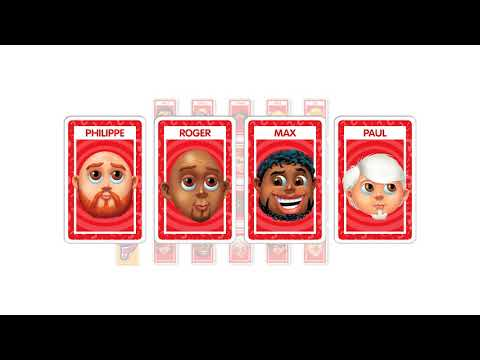
\includegraphics[scale=1]{img.jpg}   % insertion d'une image
\end{center}

\tableofcontents

\begin{abstract}     % Résumé du travail

  \emph{Description très succinte du problème et des différentes étapes de réalisation}

\end{abstract}



\section{Étape 2 : aider  à la saisie  des personnages}
\subsection{Description du problème: format des données et du résultat}
Premièrement, au début de la programmation, nous avions eu deux choix de concept pour l'attribution des caractéristiques aux personnages depuis l'interface:
\begin{itemize}
\item {Saisir manuellement (au clavier) chaque attributs, valeurs de chaque personnages}
\item {Créer les attributs et les valeurs associées, les stockers, puis les attribuer aux personnages en les sélectionnant} 
\end{itemize}
Comme les deux concepts possédaient des avantages et des inconvénients, nous avions décidé d'établir la liste de celles-ci afin de déterminer la meilleure des deux.
\begin{itemize}
\item {Pour la saisie manuelle :}
\end{itemize}

L'avantage :\\  
  - Développement d'apparence plus simple (peu de fonction à implémenter)\\

Les inconvénients :\\
  - Malgré la possibilité de vérifier les occurrences par comparaison orthographique, un "non" != "Non" != "Nope" donc possibilité d'occurence\\
  - Dans le cas d'une envie de modifier ou de supprimer un attribut ou une valeur, il faudrait apporter la modification manuellement pour chaque personnage\\
  - Complexifie les méthodes de vérification de la validité des données\\
  - Saisie inconfortable des caractéristiques
\begin{itemize}
\item {Pour la saisie des caractéristiques et leur attribution aux personnage par simple selection :}
\end{itemize}

Les avantages :\\
- Vérification de la validité des données plus simple (unicité des caractéristiques des personnages)\\
- Modification et de suppression des caractéristiques plus confortable et rapide\\

(!) Possibilité d'attribuer automatiquement les attributs déjà créés aux personnages\\

(!) Lors de la modification ou de la suppression d'un attribut ou d'une valeur, chaque personnage ayant cet attribut ou cette valeur recevra une modification automatique au niveau de sa liste de caractéristique\\
            
Les inconvénients :\\
- Malgré la possibilité de vérifier les occurrences par comparaison orthographique, un "non" != "Non" != "Nope" donc possibilité d'occurence\\
- Complexification du développement\\

(!) Création d'une class de type fenêtre pour la création et la modification des caractéristiques\\

(!) Création d'une class de type fenêtre pour l'attribution des valeurs aux attributs des personnages\\              

Après reflexion, nous avions alors opté pour le deuxième concept en raison de fait que malgré la complexité du codage, le générateur serait beaucoup plus agréable à utiliser et de meilleur qualité.\\  \\

Deuxièmement, après s'être mis d'accord sur la manière de saisie des données, il n'y avait plus qu'à réfléchir 
sur la manière de récupérer les données de chaque personnage.\\
Comme les paramètres de configuration de l'interface et le nom du plateau du qui-es-ce sont contenus directement dans les attributs du générateur, il à été facile de les récolter. 
Cependant, les personnages sont des objets de class et que leurs données ont été placées dans leurs attributs, nous avions alors implementé une fonction parcourant les personnages un à un avec leurs attributs. Au fur et à mesure, la fonction 
récolter alors leurs données sous la forme d'une String, et lorsque tout les personnages ont été parcouru,
les données des personnages et de la configuration de l'interface du qui-es-ce sont écrites dans un fichier Json généré automatiquement et dont le nom est donnée en fonction du nom du dossier contenant les images des différents personnages.

\subsection{Scénario des interactions avec l'utilisateur}
\begin{enumerate}
\item L'utilisateur exécute le programme : 
\begin{itemize}
    \item (sans sauvegarde) il saisit la commande pour exécuter le programme suivit du chemin vers les images
    \item (avec sauvegarde) il saisit la commande pour exécuter le programme suivit de l'option -save
\end{itemize}
\item Le main initialise l'interface
\item L'utilisateur configure l'interface avec les entry :
\begin{itemize}
    \item Il saisie des dimensions du plateau 
    \item Il saisie de la taille des images représentant les personnages
    \item Il saisie l'espacement entre les images
\end{itemize}

(!) Le générateur affiche d'un messages d'erreur si les dimensions de la grille ne conviennent pas, si la taille d'image est trop grande ou si l'espacement entre les images est trop grand
    
\item L'utilisateur crée les caractéristiques avec le bouton "configuration Attributs"
\item Le générateur affiche une nouvelle fenêtre permettant à l'utilisateur de créer les caractéristiques 
\begin{itemize}
    \item l'utilisateur créé / modifie ou supprime des attributs et les valeurs correspondant
\end{itemize}

(!) affichage d'une erreur s'il y a la création d'un attribut déjà existant\\

(!) affichage d'une erreur si la modification du nom d'un attribut correspond à un autre\\

(!) affiche une demande de confirmation si vous effectué une modification et affichage d'un avertissement si vous voulez supprimer un attribut ou une valeur
\item L'utilisateur affiche l'aperçu du plateau en cliquant avec le bouton "Aperçu"
\item L'utilisateur caractérise les personnages du plateau :
\begin{itemize}
    \item Clique sur l'image d'un des personnage sur l'aperçu du plateau 
    \item Le générateur affiche les attributs existant
    \item Selection des valeurs correspondant aux attributs du personnage et valide la selection 
\end{itemize}

(!) affichage d'une erreur si le dictionnaire description du personnage n'est pas unique

\begin{itemize}
    \item Répétition du même processus pour tout les personnages du plateau
\end{itemize}

\item Le générateur verifi la validité du plateau :
\begin{itemize}
    \item Il vérifie si toutes les caractéristiques de chaque personnage ont été attribuées d'une ou de plusieurs valeurs 
\end{itemize}

(!) affichage d'un message d'erreur si des personnages ont été mal caractérisés (application d'un filtre rouge sur l'image des personnage mais caractérisés / application d'un filtre vert dans le cas contraire)

  \begin{itemize}
    \item Si tout a été correctement fait, le générateur affiche un message indiquant la génération du fichier .json
\end{itemize}
\end{enumerate}


\end{document}

